%%%%%%%%%%%%%%%%%%%%%%%%%%%%%%%%%%%%%%%%%
% a0poster Portrait Poster
% LaTeX Template
% Version 1.0 (22/06/13)
%
% The a0poster class was created by:
% Gerlinde Kettl and Matthias Weiser (tex@kettl.de)
% 
% This template has been downloaded from:
% http://www.LaTeXTemplates.com
%
% License:
% CC BY-NC-SA 3.0 (http://creativecommons.org/licenses/by-nc-sa/3.0/)
%
%%%%%%%%%%%%%%%%%%%%%%%%%%%%%%%%%%%%%%%%%

%----------------------------------------------------------------------------------------
%	PACKAGES AND OTHER DOCUMENT CONFIGURATIONS
%----------------------------------------------------------------------------------------

\documentclass[portrait,a1]{a0poster}

\usepackage{multicol} % This is so we can have multiple columns of text side-by-side
\columnsep=100pt % This is the amount of white space between the columns in the poster
\columnseprule=3pt % This is the thickness of the black line between the columns in the poster

\usepackage[svgnames]{xcolor} % Specify colors by their 'svgnames', for a full list of all colors available see here: http://www.latextemplates.com/svgnames-colors

%x\usepackage{times} % Use the times font
\usepackage{palatino} % Uncomment to use the Palatino font

\usepackage{graphicx} % Required for including images
\graphicspath{{figures/}} % Location of the graphics files
\usepackage{booktabs} % Top and bottom rules for table
\usepackage[font=small,labelfont=bf]{caption} % Required for specifying captions to tables and figures
\usepackage{amsfonts, amsmath, amsthm, amssymb} % For math fonts, symbols and environments
\usepackage{wrapfig} % Allows wrapping text around tables and figures
%\usepackage{subfig}
\usepackage{float}
\usepackage[it]{subfigure}
\usepackage{epstopdf}
 \usepackage{tabularx}

\begin{document}

%----------------------------------------------------------------------------------------
%	POSTER HEADER 
%----------------------------------------------------------------------------------------

% The header is divided into two boxes:
% The first is 75% wide and houses the title, subtitle, names, university/organization and contact information
% The second is 25% wide and houses a logo for your university/organization or a photo of you
% The widths of these boxes can be easily edited to accommodate your content as you see fit



\begin{minipage}[b]{0.85\linewidth}
\Huge \color{NavyBlue} \textbf{Hierarchical Controller Architecture} \color{Black}\\[0.5cm] % Title
\Huge\color{NavyBlue}\text{in Software Defined Networks}\\[1cm] % Subtitle
\Large \text{Gourav Khaneja, Sweta Seethamraju \& Praveen Kumar}\\[0.5cm] % Author(s)

%\huge University and Department Name\\[0.4cm] % University/organization
%\Large \texttt{john@LaTeXTemplates.com} --- 1 (000) 111 1111\\
\end{minipage}
%
\begin{minipage}[b]{0.15\linewidth}

\includegraphics[scale=0.8]{UIUC_logo.png}\\
\end{minipage}


\vspace{-1cm} % A bit of extra whitespace between the header and poster content

%----------------------------------------------------------------------------------------

\begin{multicols}{2} % This is how many columns your poster will be broken into, a portrait poster is generally split into 2 columns



\color{DarkSlateGray}
Typical Control plane architecture in SDN involves multiple peer controllers, managing subset of network, but keeping a global view of the network.

\color{SaddleBrown}% DarkSlateGray color for the rest of the content
\section*{PROBLEMS}
\color{DarkSlateGray}

\begin{itemize}
    \item Replication of entire network state requires huge communication overhead: hinders scalability of the system
    \item Network inconsistency degrades the performance of control application
    \item Scalability of global network view itself
\end{itemize}


\color{SaddleBrown}
\section*{PROPOSED SOLUTION}
\color{DarkSlateGray}

\textbf{Switch Abstraction}
\begin{itemize}
    \item A controller creates an abstract switch representing the underlying managed network.
    \item A controller exposes "OpenFlow" API to manage the abstract switch by other (parent) controller.
    \item OpenFlow messages are translated between parent controller and underlying network. \\
\end{itemize}

\textbf{Hierarchical arrangement}
\begin{itemize}
    \item Controllers are arranged in a tree structure over the network using switch abstraction.
    \item Controllers do not keep a global view of network, but only the part which they control.
    \item Local application and network events are shielded from upper layer controllers.
\end{itemize}

\begin{figure}[H]
\centering
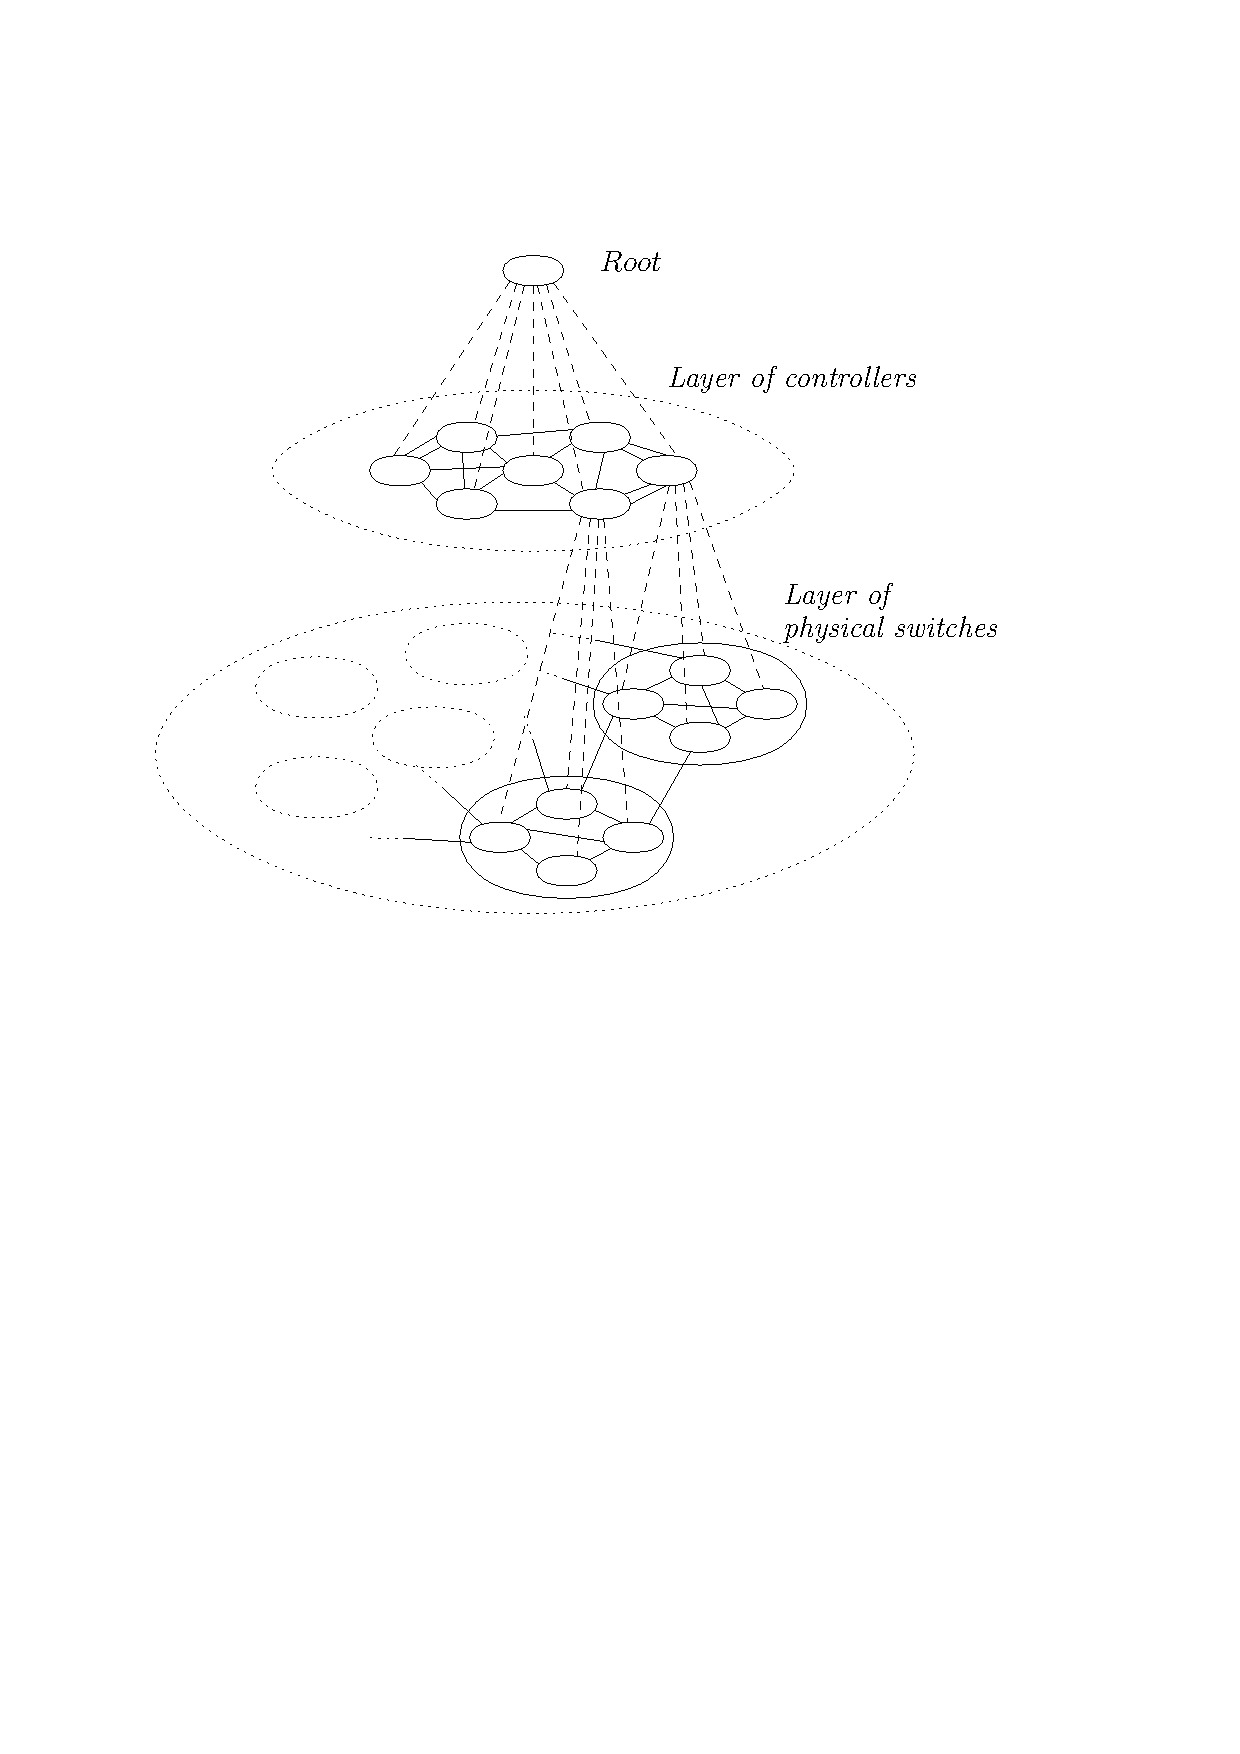
\includegraphics[scale=1.9]{hierarchy}
\caption{Hierarchical arrangement of controllers}
\label{fig:hierarchy}
\end{figure}


\textbf{Pros}
\begin{itemize}
    \item Reduces replication overhead
    \item Minimizes network inconsistency
    \item Enables smooth transition across management barriers
\end{itemize}
\textbf{Price we pay}  \\
Sub-optimality for inter-domain operations. How much is the deviation from optimality ?


%------------------------------------------------




%Gourav - I'm starting from here onwards: 
%----------------------------------------------------------------------------------------
%	RESULTS 
%----------------------------------------------------------------------------------------
\color{SaddleBrown}
\section*{EXPERIMENTAL SETUP}
\color{DarkSlateGray}
\begin{itemize}
%\item We simulated a dummy control application on both hierarchical and flat controller architectures, with same network topology and flow arrival distribution.
\item Flow data (6000 MapReduce jobs) was generated by sampling historical Hadoop traces on a 600 machine cluster at Facebook (1 million jobs). A dummy MapReduce application choses directory, map and reduce nodes randomly for each job.
\item Topology: 600 hosts connected through a network of 200 switches and 10 Gbps links. The cluster is divided into 10 equally-sized control domains.
\item TE-cum-routing control application: When a new flow arrives, it finds the path with minimum maximum utilization. If multiple such paths exist (which is frequently the case, due to a large network), shortest path (in term of number of hops) is chosen.
\end{itemize}

\color{SaddleBrown}
\section*{METRICS}
\color{DarkSlateGray}
\begin{itemize}
\item Path length (number of hops) of the routes assigned to flows.
\item Maximum link utilization of the path assigned to flows.
\item Communication overhead (number of messages exchanged between controllers) for setting up routes for flows.   
\end{itemize}



%\begin{center}\vspace{1cm}
%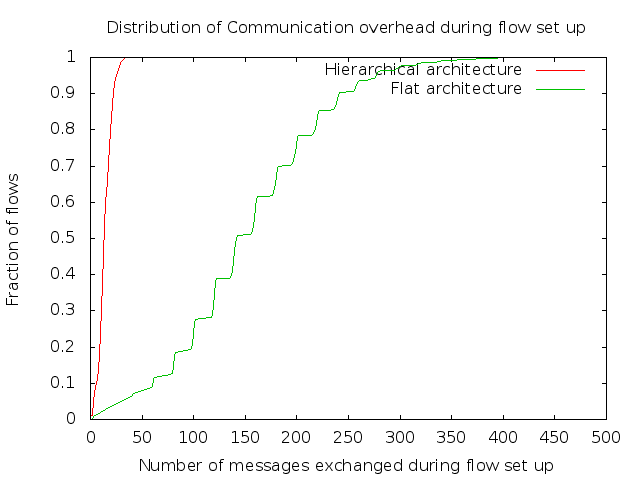
\includegraphics[width=0.8\linewidth]{msg}
%\captionof{figure}{\color{Green} Per flow communication overhead}
%\label{fig:msg}
%\end{center}\vspace{1cm}
\begin{figure}[H]
\centering
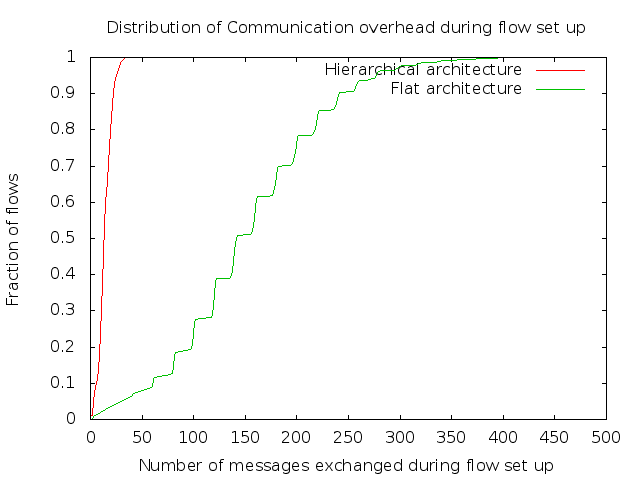
\includegraphics[scale=01]{msg}
\caption{Per flow communication overhead}
\label{fig:msg}
\end{figure}


%\begin{center}\vspace{1cm}
%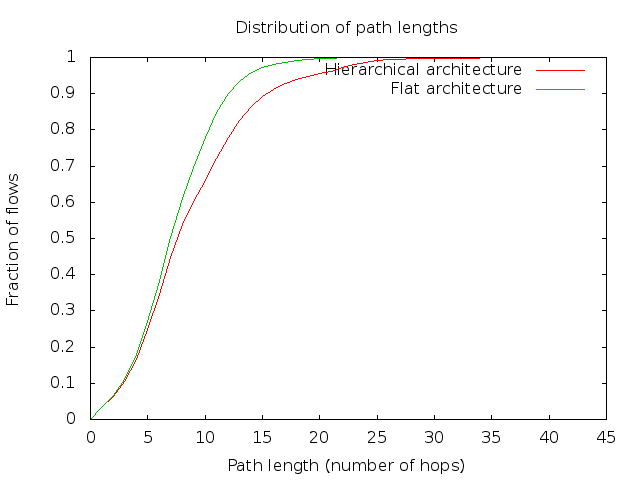
\includegraphics[width=0.5\linewidth]{path}
%\captionof{figure}{\color{Green} Path length (number of hops) assigned to flows}
%\end{center}\vspace{1cm}

%\begin{center}\vspace{1cm}
%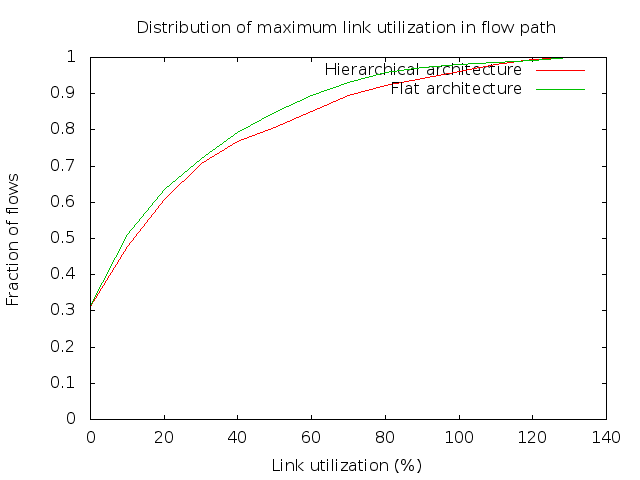
\includegraphics[width=0.5\linewidth]{util}
%\captionof{figure}{\color{Green} Maximum link utilization encountered by flows}
%\end{center}\vspace{1cm}

\begin{figure}[H]
  \begin{center}  
    \subfigure[Path length]{\label{fig:path}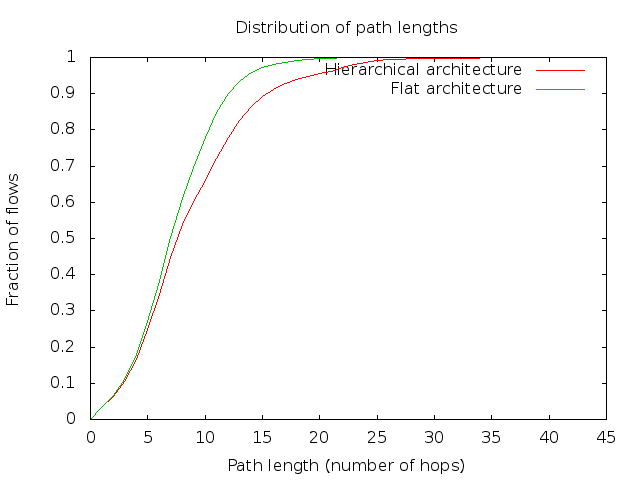
\includegraphics[scale=0.55]{path.png}} 
    \subfigure[Maximum link utilization]{\label{fig:util}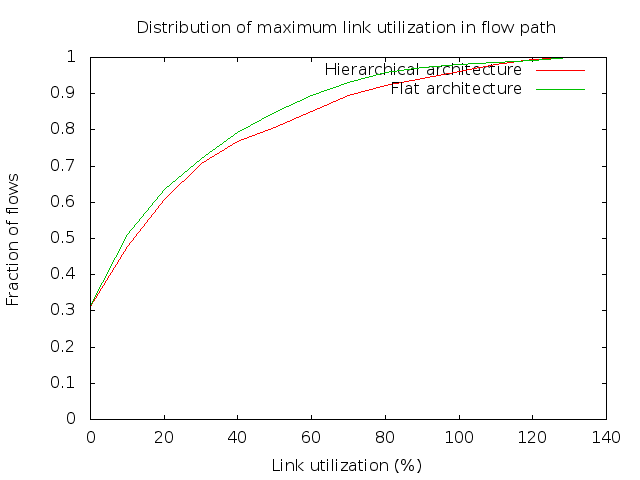
\includegraphics[scale=0.55]{util.png}} 
  \end{center}
\caption{Application performance}
\end{figure}

\color{SaddleBrown}
\section*{RESULTS}
\color{DarkSlateGray}
Hierarchical architecture reduces communication overhead (Figure \ref{fig:msg}) by an order of magnitude while compromising modestly on optimality: shortest path length (17.4\%) (Figure \ref{fig:path}) and minimum maximum link utilization (12.8\%) (Figure \ref{fig:util}).

%----------------------------------------------------------------------------------------
%	CONCLUSIONS
%----------------------------------------------------------------------------------------

\color{SaddleBrown} % SaddleBrown color for the conclusions to make them stand out

%\section*{CONCLUSION}


\color{DarkSlateGray} % Set the color back to DarkSlateGray for the rest of the content

%----------------------------------------------------------------------------------------
%	FORTHCOMING RESEARCH
%----------------------------------------------------------------------------------------

%\section*{Forthcoming Research}



 %----------------------------------------------------------------------------------------
%	REFERENCES
%----------------------------------------------------------------------------------------
\color{SaddleBrown}
\section*{RESOURCES}
\color{DarkSlateGray}
https://github.com/MugiwaraLuffy/ACN/ \\
https://github.com/SWIMProjectUCB/SWIM
%\nocite{*} % Print all references regardless of whether they were cited in the poster or not
%\bibliographystyle{plain} % Plain referencing style
%\bibliography{sample} % Use the example bibliography file sample.bib

%----------------------------------------------------------------------------------------
%	ACKNOWLEDGEMENTS
%----------------------------------------------------------------------------------------



%----------------------------------------------------------------------------------------

\end{multicols}
\end{document}
